
\section{Wall-Crossing at Stress Boundaries}\label{sec:wall}
Eight stress-boundary wall types partition $\Theta_{\mathrm{peg}}$ (\S\ref{sec:walltypes}). Across each wall the co-movement covariance jumps by a rank-one term supported on the affected coins (Assumption~\ref{ass:wallcrossing}), and the correlation matrix inherits that jump through the normalising map of \S\ref{sec:rigidity}. This section states the assumption, derives its consequences for correlations, and maps the eight historical de-peg episodes of 2020--2025 onto the wall types (\S\ref{sec:ninewalls}).

\subsection{Wall types}\label{sec:walltypes}
Four of the eight walls are equalities between a continuous structural parameter and a threshold ($W_1$, $W_2$, $W_7$, $W_8$); the other four are discrete transitions ($W_3$--$W_6$). \S\ref{sec:chambers} records why both kinds are kept in one list.
\begin{itemize}[leftmargin=1.8em]
\item[$W_1$] \emph{Backing-ratio}: $\rho_i = 1$; redemption arbitrage fails to clear at par (canonical: DAI, 12 March 2020).
\item[$W_2$] \emph{Oracle-deviation}: $|O_i - 1| = \delta_*$ at the halt threshold (canonical: FDUSD, mid-2024).
\item[$W_3$] \emph{Redemption-gate}: gate flips \texttt{open}$\to$\texttt{gated/halted} at a queue-depth threshold (canonical: UST May 2022; USDT July 2022).
\item[$W_4$] \emph{Custody}: custodian solvency event. Sub-types $W_4$-\texttt{bank} (regulated-bank; canonical: USDC/SVB, 11 March 2023) and $W_4$-\texttt{cex} (CEX/crypto custodian; canonical: FTX contagion, 08--14 November 2022).
\item[$W_5$] \emph{Bridge}: cross-chain bridge exploit/freeze isolates supply (canonical: second-order episodes on wrapped stablecoins).
\item[$W_6$] \emph{Regulatory}: regulator-forced wind-down / freeze (canonical: NY DFS $\to$ Paxos/BUSD, February 2023).
\item[$W_7$] \emph{Funding-rate}: delta-neutral synthetic issuer's perpetual-basis sign/magnitude change stresses the peg-arbitrage cycle (canonical: USDe, April--May 2024; max daily deviation $59$ bp on 2024-05-02---a marginal threshold crossing at the boundary $\varepsilon = 50$ bp). We record $W_7$ as a threshold-crossing wall of low peg-deviation intensity; the wall taxonomy applies to the local (small-signal) regime, and the amplitude of the rank-one lift of Assumption~\ref{ass:wallcrossing} is attenuated as the deviation approaches the threshold from above.
\item[$W_8$] \emph{Interest-rate / PSM}: interest-rate-driven coin with PSM buffer holds structural sub-peg when spread does not clear the buffer (canonical: GHO, 18 December 2024, closing price \$0.8085 on DeFiLlama daily snapshot, i.e., $\approx 19\%$ sub-peg).
\end{itemize}

Figure~\ref{fig:wall} illustrates the resulting chamber/wall geometry on the two continuous coordinates $(\rho, \delta)$ that carry $W_1$ and $W_2$; discrete walls $W_3$--$W_6, W_8$ appear as external annotations, and the funding-rate wall $W_7$, being one-sided in the basis, is absorbed into the boundary behavior of the $\rho$ axis.

\begin{figure}[H]
\centering
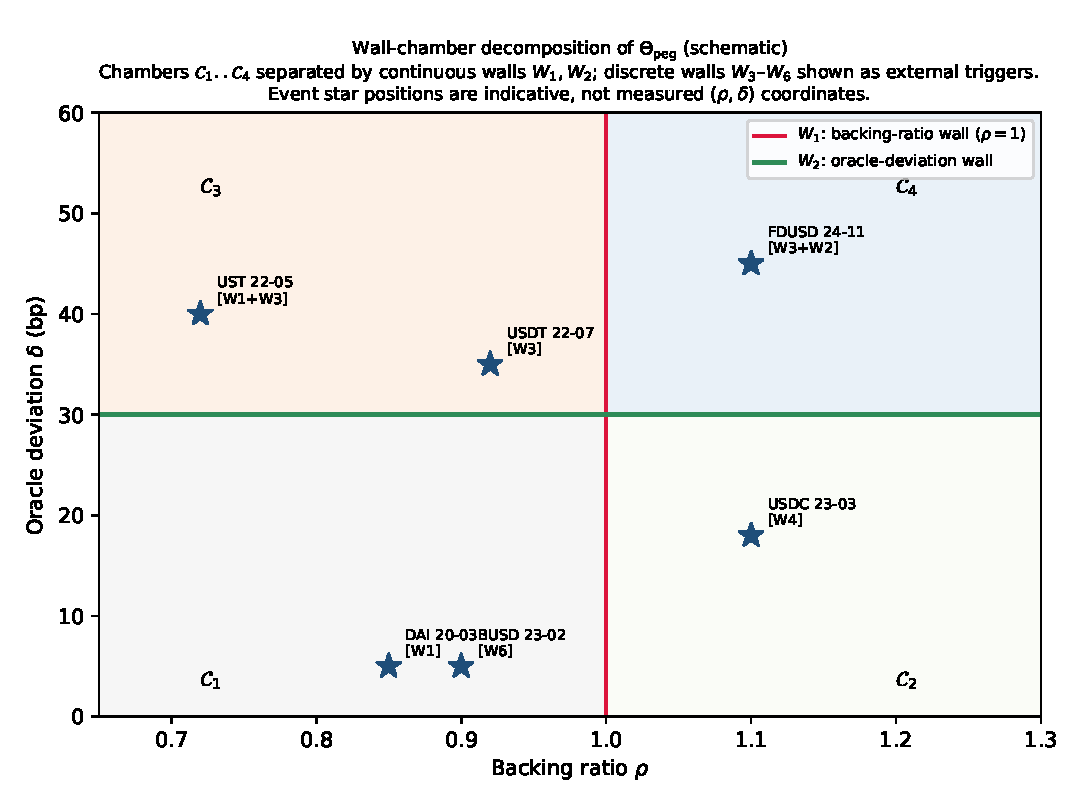
\includegraphics[width=0.78\textwidth]{figs/fig1_wall_chamber}
\caption{Wall-chamber decomposition of the peg-preserving parameter space $\Theta_{\mathrm{peg}}$ projected to the $(\rho, \delta)$-plane, drawn as a schematic illustration of the chamber/wall geometry. Continuous walls $W_1$ (backing-ratio, red) and $W_2$ (oracle-deviation, green) carve out four smooth chambers in this projection; the discrete triggers $W_3$--$W_6$ are annotated as external events, and the two further continuous walls $W_7$ and $W_8$ act on coordinates outside the $(\rho,\delta)$ plane and are not drawn.}
\label{fig:wall}
\end{figure}

\subsection{The crossing law}\label{sec:ks}
\begin{assumption}[Rank-one wall crossing, H2]\label{ass:wallcrossing}
Fix a wall $W \subset \Wpeg$ separating two adjacent chambers, and write $\Covit^\mp := \Covit(\theta^\mp)$ for the co-movement covariance matrices of Definition~\ref{def:intensity} on the two sides. Then
\begin{equation}\label{eq:wall-crossing}
\Covit^+ - \Covit^- = \sigma_W \sum_{\gamma \in \Gamma_W} \Omit(\gamma) \, v_\gamma v_\gamma^\top ,
\end{equation}
where $\Gamma_W$ is a finite index set of \emph{de-peg channels} active at $W$, $\Omit(\gamma) \in \mathbb{R}$ is a signed weight attached to channel $\gamma$, $v_\gamma \in \mathbb{R}^N$ is a direction vector supported on the coins that channel $\gamma$ affects, and $\sigma_W > 0$ is a single positive scalar amplitude.
\end{assumption}

\begin{assumption}[Block support, H3]\label{ass:support}
For each wall $W$ crossed by an episode with a multi-coin failure channel, the directions $\{v_\gamma\}_{\gamma \in \Gamma_W}$ span the indicator directions of a single group of coins $B_W$, the \emph{wall-affected block}: the coins that share the failing custodian, the crossing oracle, or the gating issuer as the case may be. Coins outside $B_W$ carry zero weight.
\end{assumption}

The shape of \eqref{eq:wall-crossing} is the shape of the Kontsevich--Soibelman wall-crossing formula \citep{KontsevichSoibelman2008}, which takes a product over the charges whose central charges change sign across a wall and which, in the setting where it applies, produces exactly a signed sum of rank-one terms supported on the coins those charges carry. That analogy is why the form is a natural one to posit; nothing below depends on the analogy being true, and \S\ref{sec:what-is-assumed} records why the paper states the law rather than derives it. Two features of the original are not transported. $\Omit(\gamma)$ is not claimed to be an integer, since only the product $\sigma_W\Omit(\gamma)$ is ever identified and integrality would therefore carry no empirical content. And no sign restriction is placed on $\Omit(\gamma)$, which means the right-hand side of \eqref{eq:wall-crossing} is a general symmetric matrix rather than a positive semidefinite one. The crossing law therefore fixes the \emph{support} of the jump but not its direction: the direction enters through the effective amplitude $a=\sigma_W\Omit(\gamma_0)$ of Remark~\ref{rem:small-cases}, and the prediction tested in \S\ref{sec:empirical} is that $a>0$ for the events in the sample. That is a substantive empirical claim, not a consequence of the assumptions.

\begin{corollary}[The induced correlation jump has zero diagonal]\label{cor:wall-jump}
Let $\Deltait_R := \Sigmait^+ - \Sigmait^-$ be the induced correlation jump \eqref{eq:corr-jump}. Then $\Deltait_R{}_{ii} = 0$ for every $i$: the correlation jump is tangent to the manifold of correlation matrices.
\end{corollary}
\begin{proof}
By \eqref{eq:normalised-corr}, $\Sigmait^+_{ii} = \Sigmait^-_{ii} = 1$ for every $i$, on both sides of the wall. Hence $\Deltait_R{}_{ii} = 1 - 1 = 0$. No clipping, projection, or post-hoc renormalisation is involved. This is why the crossing law is stated on $\Covit$ (Remark~\ref{rem:why-cov}): the same rank-one increment, imposed directly on $\Sigmait$, would require $\Sigmait^+_{ii}-\Sigmait^-_{ii}=a>0$ against the unit diagonal, and the identity would be false as stated.
\end{proof}

\begin{remark}[Explicit two-coin case: the jump lives on the covariance, and its correlation image has zero diagonal]\label{rem:small-cases}
Take a single-channel wall $\Gamma_W = \{\gamma_0\}$ with $\Omit(\gamma_0) = 1$ and $v_{\gamma_0} = e_i + e_j$, so the channel affects stablecoins $i$ and $j$ symmetrically. Writing $a := \sigma_W > 0$, the crossing law~\eqref{eq:wall-crossing} reduces on the block $\{i,j\}$ to
\begin{equation}\label{eq:block-jump}
\Covit^+_{k\ell} - \Covit^-_{k\ell} = a\,\mathbf{1}_{k \in \{i,j\}}\,\mathbf{1}_{\ell \in \{i,j\}},
\end{equation}
with all entries outside the block unchanged: the covariance block jumps by $a\begin{pmatrix}1&1\\1&1\end{pmatrix}$.

The corresponding change in the \emph{correlation} matrix is not \eqref{eq:block-jump}. Since $\Sigmait = D^{-1/2}\Covit D^{-1/2}$, one has $\Sigmait^\pm_{ii} = 1$ by construction on both sides, so
\begin{equation}\label{eq:block-jump-corr}
\Sigmait^+_{ii} - \Sigmait^-_{ii} = 0 \quad\text{for } i \in \{i,j\},
\end{equation}
while the off-diagonal entry moves by
\begin{equation}\label{eq:block-jump-corr-off}
\Sigmait^+_{ij} - \Sigmait^-_{ij}
= \frac{\Covit^-_{ij} + a}{\sqrt{(\Covit^-_{ii}+a)(\Covit^-_{jj}+a)}} - \frac{\Covit^-_{ij}}{\sqrt{\Covit^-_{ii}\,\Covit^-_{jj}}} .
\end{equation}
The diagonal of the induced correlation jump therefore vanishes identically---not by clipping or by renormalising after the fact, but because the normalisation \eqref{eq:normalised-corr} assigns the diagonal rather than computing it.

\emph{Sign.} Write $p:=\Covit^-_{ij}$, $X:=\Covit^-_{ii}$, $Y:=\Covit^-_{jj}$. Differentiating \eqref{eq:block-jump-corr-off} at $a=0$ gives
\[
\frac{d}{da}\Big|_{a=0}\bigl(\Sigmait^+_{ij}-\Sigmait^-_{ij}\bigr)
= \frac{1}{\sqrt{XY}} - \frac{p}{2}\left(\frac{1}{X}+\frac{1}{Y}\right)\frac{1}{\sqrt{XY}}
= \frac{1}{\sqrt{XY}}\left(1 - \frac{p\,(X+Y)}{2XY}\right),
\]
so the block entry rises near the wall precisely when
\begin{equation}\label{eq:block-sign}
p \;<\; \frac{2XY}{X+Y},
\end{equation}
the harmonic mean of the two variances. By the arithmetic--geometric mean inequality that harmonic mean is at most the geometric mean $\sqrt{XY}$, with equality exactly when $X=Y$; and $|p|\le\sqrt{XY}$ holds because the covariance matrix is positive semidefinite. The two facts together give a clean reading of \eqref{eq:block-sign}: when the two coins have equal variances the condition holds for every admissible $p$, while when the variances are unequal the condition can fail only if the pair is both strongly correlated and strongly heteroscedastic. The leading coefficient is therefore \emph{not} $a/\sqrt{XY}$ in general, and writing it that way is the $p=0$ special case. On the primary event of \S\ref{sec:empirical} the pre-event block correlations are at most $0.20$ in absolute value, comfortably inside the region where \eqref{eq:block-sign} holds and where the $p$-free leading term is accurate to a few percent.

\emph{Magnitude against the cross pairs.} The behaviour of a pair with one coin inside the block and one outside is different in sign. Take $i$ in the block and $k$ outside it. Then $\Covit^+_{ik} = \Covit^-_{ik}$ but $\Covit^+_{ii} = \Covit^-_{ii}+a$, so
\begin{equation}\label{eq:cross-jump-corr}
\Sigmait^+_{ik} - \Sigmait^-_{ik}
= \Covit^-_{ik}\cdot\frac{1}{\sqrt{\Covit^-_{kk}}}\left(\frac{1}{\sqrt{\Covit^-_{ii}+a}} - \frac{1}{\sqrt{\Covit^-_{ii}}}\right)
= -\frac{a\,\Covit^-_{ik}}{2\,(\Covit^-_{ii})^{3/2}\sqrt{\Covit^-_{kk}}} + O(a^2).
\end{equation}
The bracket is strictly negative, so this entry moves in the direction \emph{opposite} to the pre-event covariance and vanishes exactly when $\Covit^-_{ik}=0$. Its size relative to the block entry of \eqref{eq:block-jump-corr-off} is of order $|\Covit^-_{ik}|/(2\Covit^-_{ii})$, which is small when the pre-event cross-covariance is small relative to the block coin's variance---the empirically relevant case---but which is not bounded away from the block term in general. The correlation image of a wall crossing is therefore not supported on the block alone; only its leading term is, and the test of \S\ref{sec:empirical} is accordingly built on the block-versus-rest contrast rather than on a claim that off-block entries are unchanged.
\end{remark}

\subsection{Nine historical wall crossings}\label{sec:ninewalls}
Each of the nine documented de-peg episodes over 2020--2025 maps to one, two, or (in the USDC-SVB case) three of the walls $W_1$--$W_8$ (Table~\ref{tab:events}).

\paragraph{Ex-ante coding discipline (identifying restriction).} The block $B_W$ of Assumption~\ref{ass:support} is fixed by the wall's structural definition---which coins share the failing custodian for $W_4$, which coins depend on the crossing oracle for $W_2$, and so on---and never by the correlation outcomes the theory predicts. Wall-type assignments in Table~\ref{tab:events} are likewise fixed by the regulator or post-mortem literature contemporaneous with (or immediately following) each event. This ex-ante coding is the identifying restriction that permits the pair-level gradient test of \S\ref{sec:gradient} to distinguish the block prediction from a purely descriptive account of crisis-wide co-movement.

\begin{table}[!ht]
\centering
\caption{Nine documented multi-stablecoin de-peg episodes over 2020--2025 and their wall-type assignments. Wall types as in \S\ref{sec:walltypes}; assignment follows the primary structural failure in the regulator and post-mortem literature (Appendix~\ref{app:data}). USDC-SVB is a triple wall following \citet{MaZengZhang2023}. The rightmost column reports whether the event delivers a multi-coin wall-affected block or a single-coin block. Only 3 of the 9 events deliver a multi-coin wall-affected block, and the pair-level gradient test of \S\ref{sec:gradient} is defined on exactly those three; the remaining six are single-coin blocks and cannot carry the test by construction (\S\ref{sec:single}).}
\label{tab:events}
\resizebox{\textwidth}{!}{%
\begin{tabular}{@{}llll@{}}
\toprule
Episode & Date & Wall(s) crossed & Block \\
\midrule
DAI Black Thursday        & 12--13 Mar 2020 & $W_1$ (backing collapse)                                                & single \\
UST/LUNA collapse         & 09--12 May 2022 & $W_1 + W_3$ (backing + gate)                                           & single \\
USDT stress episode       & 12--13 Jul 2022 & $W_3$ (queue-depth spike)                                              & single \\
FTX contagion             & 08--14 Nov 2022 & $W_4$-\texttt{cex} (CEX solvency)                                      & \textbf{multi} \\
BUSD wind-down            & 13 Feb 2023     & $W_6$ (regulatory)                                                     & single \\
USDC--SVB weekend         & 10--13 Mar 2023 & $W_4$ trigger $+$ $W_1$ transmission $+$ $W_3$ gating                  & \textbf{multi} \\
FDUSD 2024 event          & 08 Nov 2024     & $W_3 + W_2$ (gate + oracle)                                            & \textbf{multi} \\
USDe funding-stress crossing & 02 May 2024  & $W_7$ (basis compression; 59 bp)                                       & single \\
GHO structural sub-peg    & 18 Dec 2024     & $W_8$ (interest-rate / PSM)                                            & single \\
\bottomrule
\end{tabular}%
}
\end{table}

\subsection{Contrast with the Gaussian copula}\label{sec:copula-fail}
\begin{corollary}[Gaussian copula as generic-stratum smoothing]\label{cor:copula-fail}
Let $\Sigmait_G(\theta)$ denote the Gaussian copula correlation surface of \citet{Li2000}, a smooth globally defined function of $\theta \in \Bpeg$ calibrated by
\begin{center}
(CH) at each wall $W \subset \Wpeg$, $\ \Sigmait_G(\theta_W) = \tfrac{1}{2}\big(\Sigmait^+ + \Sigmait^-\big)$,
\end{center}
where $\Sigmait^\pm$ are the correlation matrices \eqref{eq:normalised-corr} on the two sides of $W$. Write
\begin{equation}\label{eq:corr-jump}
\Deltait_R := \Sigmait^+ - \Sigmait^- = D_+^{-1/2}\Covit^+ D_+^{-1/2} - D_-^{-1/2}\Covit^- D_-^{-1/2}
\end{equation}
for the \emph{induced correlation jump}, with $\Covit^\pm$ related by \eqref{eq:wall-crossing} and $D_\pm=\operatorname{diag}(\Covit^\pm)$. Then, under CH and Theorem~\ref{thm:rigidity}, the copula is a smoothing of $\Sigmait$ that annihilates the wall jump: at any wall $W \subset \Wpeg$ and any $\epsilon > 0$,
\begin{equation}\label{eq:copula-gap}
\Sigmait(\theta^\epsilon_\pm) - \Sigmait_G(\theta^\epsilon_\pm) = \pm\tfrac{1}{2}\Deltait_R + O(\epsilon).
\end{equation}
Here $\epsilon > 0$ is the parameter distance from the wall $W$ within $\Theta_{\mathrm{peg}}$ (not the peg-preservation threshold $\varepsilon = 50$ bp of Definition~\ref{def:stable}); the linearisation is valid on a neighbourhood of $W$ on which peg deviations remain within the small-signal regime, and the near-terminal UST/LUNA excursion (Appendix~\ref{app:oos}) is documented as exiting this neighbourhood.
\end{corollary}

Two structural facts about $\Deltait_R$ are used downstream. \emph{(i) Zero diagonal.} $\Sigmait^\pm_{ii}=1$ on both sides, so $\Deltait_R{}_{ii}=0$; the jump therefore lies in the tangent space of the correlation manifold. \emph{(ii) Footprint.} $\Deltait_R$ is not itself rank-one---its rank-one ancestor is the covariance jump \eqref{eq:wall-crossing}, and the normalisation~\eqref{eq:normalised-corr} is a nonlinear congruence. The normalisation also \emph{spreads} the jump beyond the block: because it moves the diagonal entry $\Covit_{ii}$ of every coin in the block, a pair with one coin inside and one outside shifts whenever $\Covit^-_{ij}\neq 0$, and by \eqref{eq:cross-jump-corr} it shifts in the \emph{opposite} direction to $\Covit^-_{ij}$. What survives in correlation space is therefore a signed footprint in three tiers: positive on block pairs (subject to the side condition \eqref{eq:block-sign}), of opposite sign on cross pairs, and identically zero on pairs outside the block. This footprint is the \emph{block signature} of the wall, in the sense introduced in \S\ref{sec:intro}, and the empirical test of \S\ref{sec:empirical} is built on it rather than on a claim of rank-one structure in $\Sigmait$.

Corollary~\ref{cor:copula-fail} makes precise the sense in which the Gaussian copula fails at stress boundaries: the failure is structural, not a matter of insufficient calibration data. The copula surface is a smooth manifold; the true correlation is locally constant on chambers and jumps across their boundaries. No amount of recalibration on smooth-chamber data can generate the wall jump. The magnitude in \eqref{eq:copula-gap} is a consequence of the midpoint calibration (CH), not of the Gaussian-copula family: any smooth surface that takes the value $\tfrac12(\Sigmait^++\Sigmait^-)$ at the wall inherits it. What extends beyond that family is the qualitative conclusion, and it needs only local continuity in $\theta$: a smooth surface cannot follow a function that is constant on chambers and jumps across their boundaries, so its distance from $\Sigmait$ is of the order of the jump and does not vanish as $\epsilon\to0$, whatever the parametric form. The same reading applies to the Ledoit--Wolf shrinkage of \citet{LedoitWolf2004} and the POET thresholded principal-orthogonal complements of \citet{FanLiaoMincheva2013}, neither of which is calibrated by (CH) and so are not claimed to satisfy \eqref{eq:copula-gap} with the constant $\tfrac12$.
